\subsection{Analyse von Schaltkreis c)}


\begin{figure}[h]
	\centering
	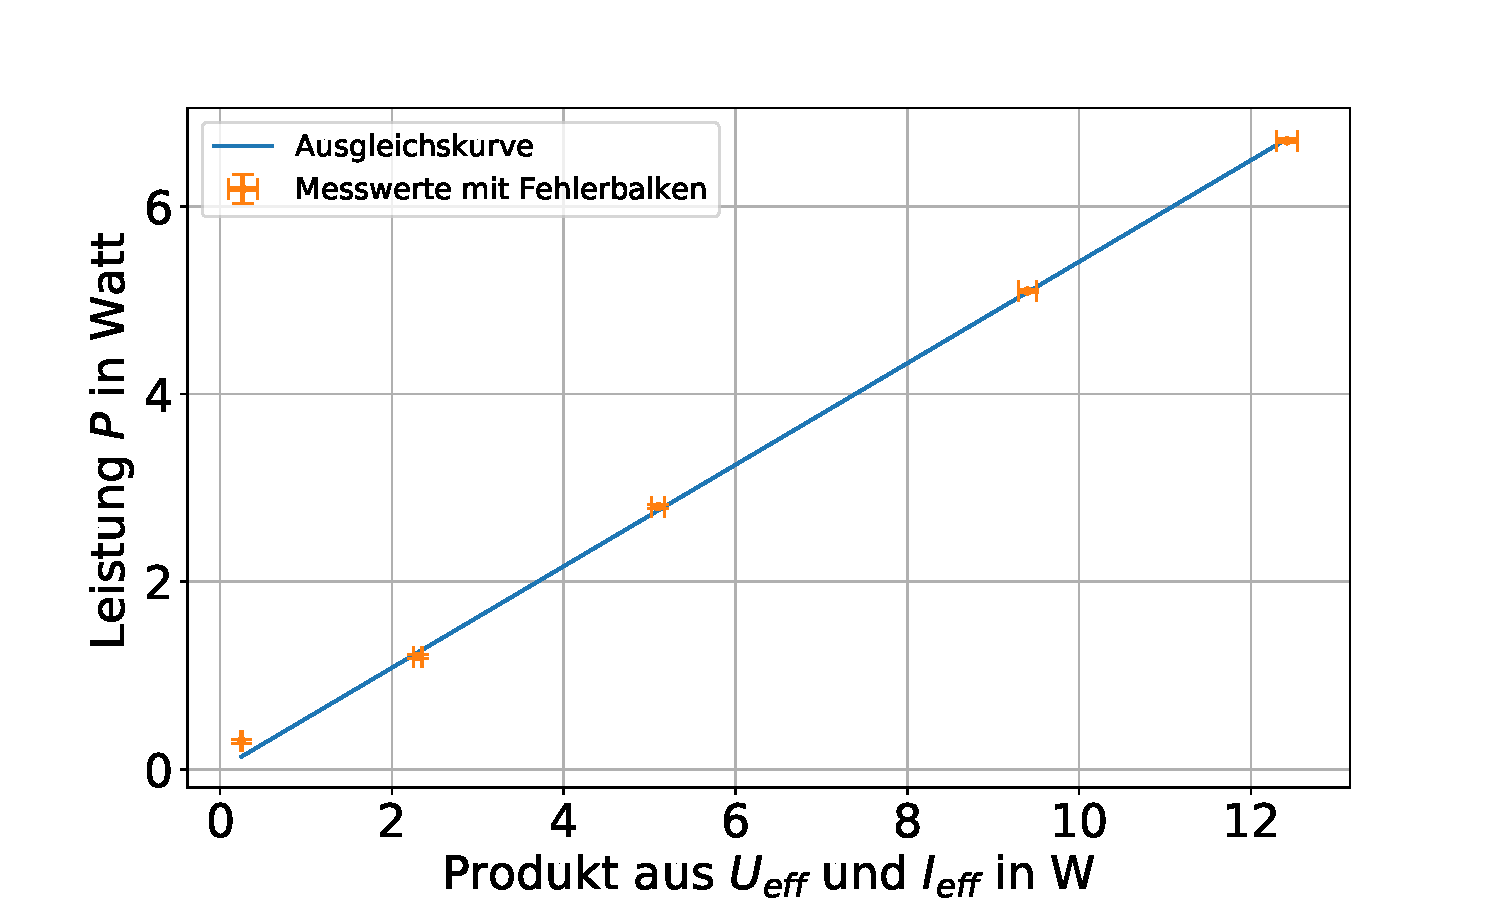
\includegraphics[width=0.9\textwidth]{res/PgegenUIK.pdf}
	\caption{Produkt aus Spannung $U$ und Strom $I$ gegen die Leistung $P$.}
	\label{fig:PgegenUIK}
\end{figure}


\begin{figure}[h]
	\centering
	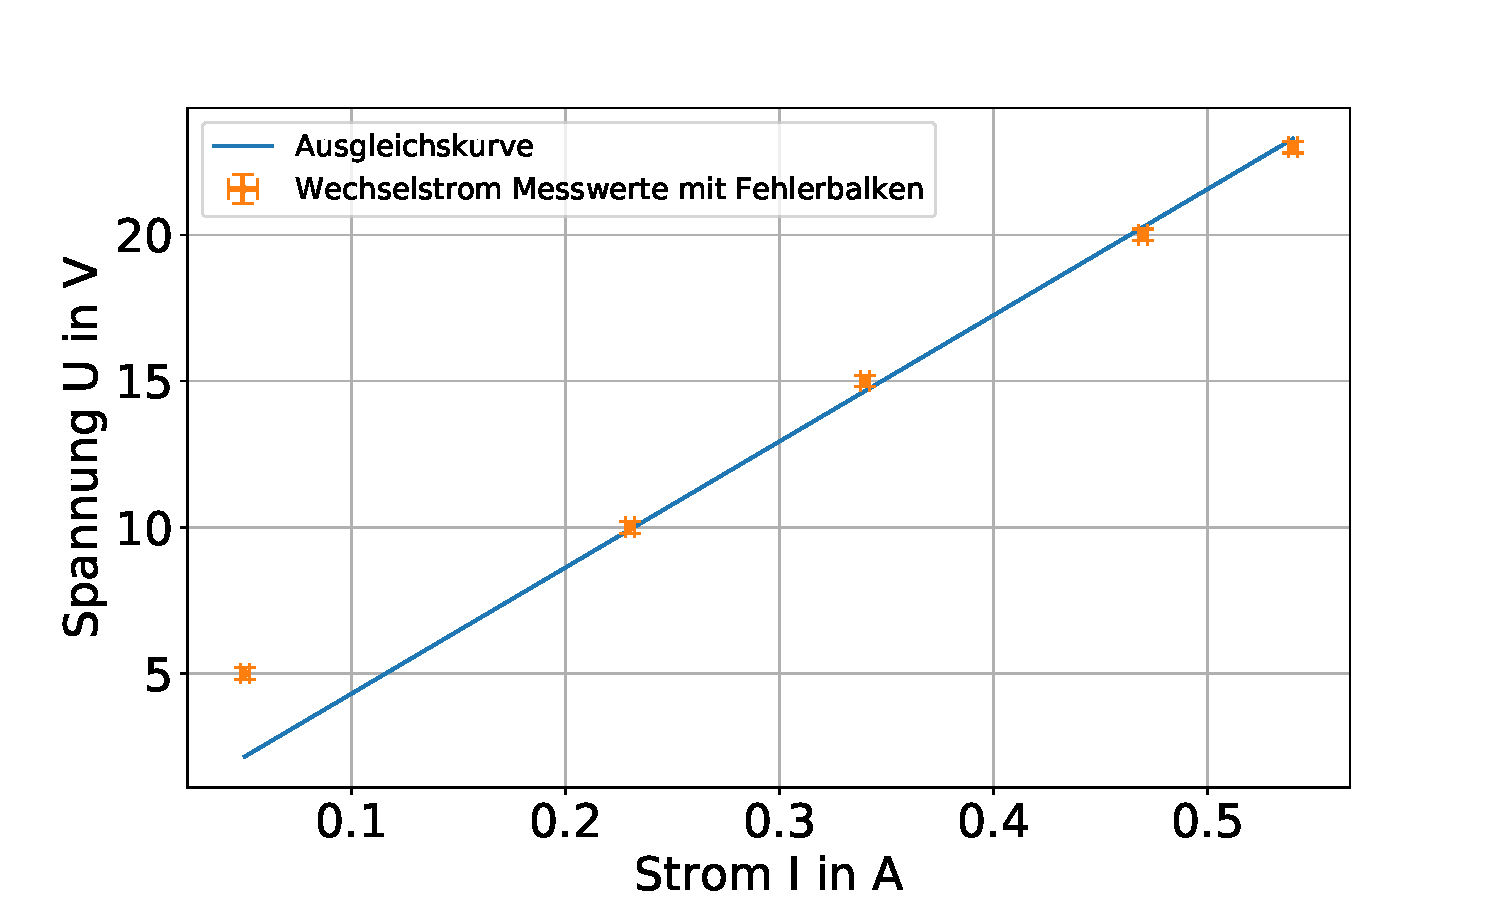
\includegraphics[width=0.9\textwidth]{res/UgegenIK.pdf}
	\caption{Spannung $U$ gegen den Strom $I$}
	\label{fig:UgegenIK}
\end{figure}


In diesem Teil des Protokossl wird die Kapazität, der Scheinwiderstand und der Phasenwinkel der schon in Kapitel \ref{kap:MethodenS} beschriebenen Schaltung c). 
Dazu wurde zum einem der Innenwiderstand $R_i$ und die Induktivität $L$ der Spule aus der Auswertung aus Kapitel \ref{kap:Spule}.
Im folgenden wird mit Hilfe der Abbildungen \ref{fig:PgegenUIK} und \ref{fig:UgegenIK}
und den folgenden Gleichungen:
\begin{align}
C=\frac{1}{\omega (\omega L+\sqrt{Z^2-R^2})}\\	
\phi = \arccos\left(\frac{\bar{P}}{U_{eff.}I_{eff.}}\right)\\
	|Z|=\frac{U_{eff.}}{I_{eff.}}\\	
\end{align}
die Kapazität $C$ des Kondensators, der Betrag des Scheinwiderstandes und der Betrag der Phase berechnet. Und das Ergebnis für den Kondensator mit dem vom Kondensator abgelesenen Wert für die Kapazität vergleichen.
Der Kondensator hatte nach Hersteller angaben eine Kapazität von \SI{60+-3.46}{µF}.
Dieser Wert liegt in der $1\sigma$-Umgebung des errechneten Wertes: \SI{57.4+-3.8}{µF} und stimmt somit gut mit dem Theoretischen Wert überein.
Um die Unsicherheiten der Werte zu erhalten wurde einmal für den Herstellerwert die von diesem angegebene Unsicherheit von $10\%$ nach Gleichung
\ref{eq:su3} abgeschätzt und die anderen Unsicherheitsrechnungen sind in \ref{kap:Unsich}
Die anderen Ergebnisse lauten:
%\begin{align}
%		\phi=SI{0.9989+-0.0006}{rad}\\
%		|Z|=SI{43.1+-3.1}{\ohm}
%\end{align}
